\documentclass{standalone}

\usepackage{tikz}
\usetikzlibrary{calc}

\begin{document}

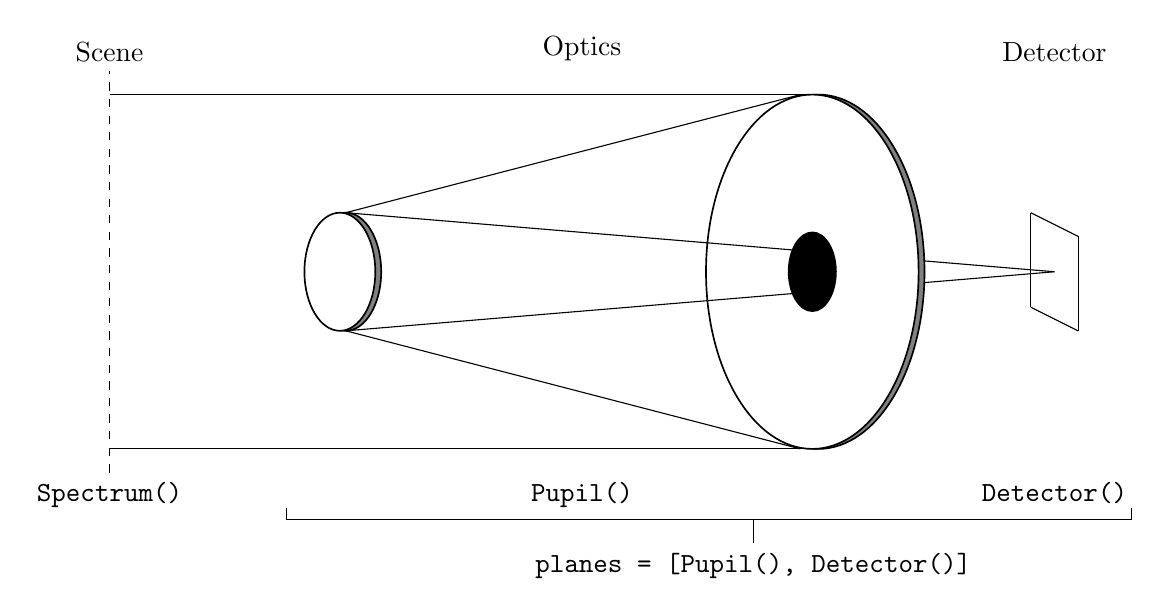
\begin{tikzpicture}[scale=1.5]

    \draw[semithick, fill=gray] (2,1.5) ellipse (0.3 and 0.5); % edge of secondary mirror
    \draw[semithick, fill=white] (1.95,1.5) ellipse (0.3 and 0.5); % front of secondary mirror


    \draw (6,1.6666) -- (8,1.5); % top hole - detector
    \draw (6,1.3333) -- (8,1.5); % bot hole - detector

    \draw[semithick, fill=gray] (6,1.5) ellipse (0.9 and 1.5); % edge of primary mirror
    \draw[semithick, fill=white] (5.95,1.5) ellipse (0.9 and 1.5); % front of primary mirror
    \draw[semithick, fill=black] (5.95,1.5) ellipse (0.2 and 0.3333); % hole in primary mirror

    \draw (0,3) -- (6,3); % top scene - pm
    \draw (5.85,3) -- (2,2); % top pm - sm
    \draw (2,2) -- (6,1.6666); % top sm - hole

    \draw (0,0) -- (6,0); % bot scene - pm
    \draw (5.85,0) -- (2,1); % bot pm - sm
    \draw (2,1) -- (6,1.3333); % bot sm - hole

    \draw (7.8,1.2) -- (7.8,2);
    \draw (7.8,2) -- (8.2,1.8);
    \draw (8.2,1) -- (8.2,1.8);
    \draw (8.2,1) -- (7.8,1.2);

    \draw[dashed] (0,-0.2) -- (0,3.2);

    \draw (1.5,-0.6) -- (8.65,-0.6);
    \draw (1.5,-0.6) -- (1.5,-0.5);
    \draw (8.65,-0.6) -- (8.65,-0.5);
    \draw (5.45,-0.6) -- (5.45,-0.8);

    \node[align=center, above] at (0,3.2) {Scene};
    \node[align=center, above] at (8,3.2) {Detector}; % (8,2.1) for just above
    \node[align=center, above] at (4,3.2) {Optics};

    \node[align=center, below] at (0,-0.2) {\texttt{Spectrum()}};
    \node[align=center, below] at (8,-0.2) {\texttt{Detector()}}; % (8,0.9) for just below
    \node[align=center, below] at (4.0,-0.2) {\texttt{Pupil()}};
    \node[align=center, below] at (5.45,-0.8) {\texttt{planes = [Pupil(), Detector()]}};
\end{tikzpicture}

\end{document}
